% !TeX root = 机械设计.tex
% ============================================================
%  第二章 机械零件的强度
%  来源：教材/机械设计《机械原理与机械设计（下）》读书笔记
%  说明：正文表述与公式均沿用原文，仅作版式与环境归类
% ============================================================
\chapter{机械零件的强度}
\label{chap:机械零件的强度}

\section{载荷与应力的分类}
\label{sec:载荷与应力的分类}

\subsection{载荷的分类}
\label{subsec:载荷的分类}

\begin{definition}[静载荷]
\label{def:静载荷}
\textbf{静载荷}：载荷的大小和方向不随时间变化或变化缓慢的载荷。
\end{definition}

\begin{definition}[变载荷]
\label{def:变载荷}
\textbf{变载荷}：载荷的大小和方向随时间变化的载荷。变载荷可分为
\begin{enumerate}
	\item 循环变载荷：
	\begin{enumerate}
		\item 稳定循环载荷；
		\item 不稳定循环载荷。
	\end{enumerate}
	\item 随机变载荷。
\end{enumerate}
\end{definition}

\subsection{应力的分类}
\label{subsec:应力的分类}

\begin{definition}[静应力]
\label{def:静应力}
\textbf{静应力}：不随时间变化或变化缓慢的应力，其随时间的变化规律如图~\ref{fig:静应力} 所示。
\end{definition}

\begin{figure}[H]
\centering
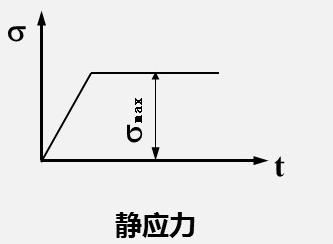
\includegraphics[width=0.52\textwidth]{Figure/静应力.png}
\caption{静应力}
\label{fig:静应力}
\end{figure}

\begin{definition}[变应力]
\label{def:变应力}
\textbf{变应力}：随时间变化的应力，可分为
\begin{enumerate}
	\item \textbf{不稳定变应力}：
	\begin{enumerate}
		\item 规律性不稳定变应力，如图~\ref{fig:规律性不稳定变应力} 所示；
		\item 随机变应力，如图~\ref{fig:随机变应力} 所示。
	\end{enumerate}
	\item \textbf{稳定循环变应力}：
	\begin{enumerate}
		\item 非对称循环变应力，如图~\ref{fig:非对称循环变应力} 所示；
		\item 脉动循环变应力，如图~\ref{fig:脉动循环变应力} 所示；
		\item 对称循环变应力，如图~\ref{fig:对称循环变应力} 所示。
	\end{enumerate}
\end{enumerate}
\end{definition}

\begin{figure}[H]
\centering
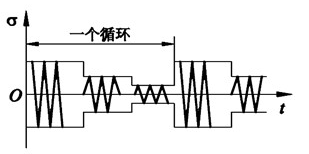
\includegraphics[width=0.6\textwidth]{Figure/规律性不稳定变应力.png}
\caption{规律性不稳定变应力}
\label{fig:规律性不稳定变应力}
\end{figure}

\begin{figure}[H]
\centering
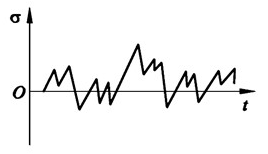
\includegraphics[width=0.55\textwidth]{Figure/随机变应力.png}
\caption{随机变应力}
\label{fig:随机变应力}
\end{figure}

\begin{figure}[H]
\centering
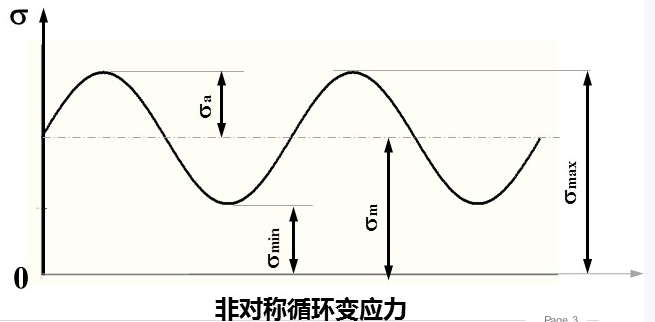
\includegraphics[width=0.72\textwidth]{Figure/非对称循环变应力.png}
\caption{非对称循环变应力}
\label{fig:非对称循环变应力}
\end{figure}

\begin{figure}[H]
\centering
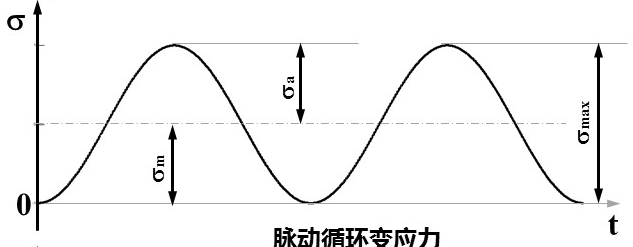
\includegraphics[width=0.68\textwidth]{Figure/脉动循环变应力.png}
\caption{脉动循环变应力}
\label{fig:脉动循环变应力}
\end{figure}

\begin{figure}[H]
\centering
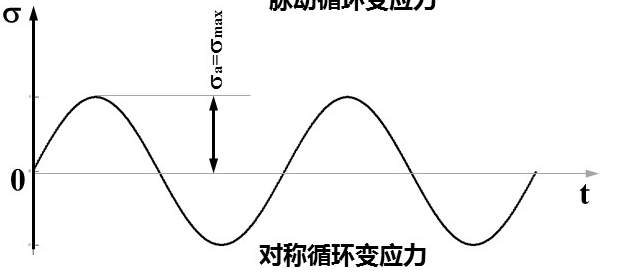
\includegraphics[width=0.68\textwidth]{Figure/对称循环变应力.png}
\caption{对称循环变应力}
\label{fig:对称循环变应力}
\end{figure}

\subsection{稳定循环变应力的基本参数}
\label{subsec:稳定循环变应力参数}

稳定循环变应力的基本参数包括最大应力 $\sigma_{\max}$、最小应力 $\sigma_{\min}$、平均应力 $\sigma_m$ 和应力幅 $\sigma_a$，其相互关系如下。

\begin{definition}[平均应力]
\label{def:平均应力}
\textbf{平均应力}是指循环变应力中静应力分量的部分，其值为
\begin{equation}
	\sigma_m = \frac{\sigma_{\max}+\sigma_{\min}}{2}
	\label{eq:强度:平均应力}
\end{equation}
\end{definition}

\begin{definition}[应力幅]
\label{def:应力幅}
\textbf{应力幅}是指循环变应力中变动应力分量的部分，其值为
\begin{equation}
	\sigma_a = \frac{\sigma_{\max}-\sigma_{\min}}{2}
	\label{eq:强度:应力幅}
\end{equation}
\end{definition}

\begin{definition}[应力循环特性（循环比）]
\label{def:应力循环特性}
\textbf{应力循环特性（循环比）}是指最小应力与最大应力之比，即
\begin{equation}
	\gamma = \frac{\sigma_{\min}}{\sigma_{\max}}, \qquad -1 < \gamma < +1
	\label{eq:强度:循环特性}
\end{equation}
\end{definition}

\begin{keybox}[脉动循环与对称循环]
脉动循环变应力：$\gamma=\dfrac{\sigma_{\min}}{\sigma_{\max}}=0$（$\sigma_{\min}=0$）；
对称循环变应力：$\gamma=\dfrac{\sigma_{\min}}{\sigma_{\max}}=-1$（$\sigma_{\max}=-\sigma_{\min}$）。
\end{keybox}

\begin{note}
静应力只能由\textcolor{red}{静载荷}产生；而变应力可能由\textcolor{red}{变载荷}产生，也可能由\textcolor{red}{静载荷}产生。对强度最不利的是\textcolor{red}{对称循环变应力}（$\gamma=-1$）。
\end{note}

\begin{figure}[H]
\centering
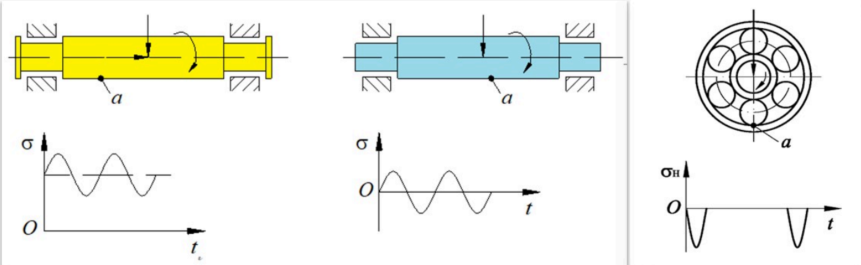
\includegraphics[width=0.6\textwidth]{Figure/静载荷动应力的例子.png}
\caption{静载荷产生动应力的例子}
\label{fig:静载荷动应力的例子}
\end{figure}

\subsection{名义应力和计算应力}
\label{subsec:名义应力和计算应力}

\begin{definition}[名义应力]
\label{def:名义应力}
\textbf{名义应力}：由名义载荷产生的应力。
\end{definition}

\begin{definition}[计算应力]
\label{def:计算应力}
\textbf{计算应力}：由计算载荷产生的应力。
\begin{equation}
	F_{ca}=KF
	\label{eq:强度:计算载荷}
\end{equation}
其中，$F_{ca}$ 为计算载荷（\emph{calculated load}），$K$ 为载荷系数（\emph{load factor}），$F$ 为名义载荷（\emph{nominal load}）。
\end{definition}

\section{静应力时机械零件的强度计算}
\label{sec:静应力时的强度计算}

\subsection{静应力下机械零件的强度}

\subsubsection{单向应力下的塑性材料零件}

按照\textcolor{red}{不发生塑性变形}的条件进行强度计算，零件危险剖面上的工作应力即为计算应力，强度条件为

\begin{theorem}[单向应力塑性材料零件的强度条件]
\label{thm:单向静应力强度}
\begin{equation}
	\begin{cases}
		\sigma_{\mathrm{ca}} \le [\sigma] = \dfrac{\sigma_{\mathrm{s}}}{[S]_\sigma} \\[2ex]
		\tau_{\mathrm{ca}} \le [\tau] = \dfrac{\tau_{\mathrm{s}}}{[S]_\tau}
	\end{cases}
	\label{eq:强度:单向静应力强度}
\end{equation}
或
\begin{equation}
	\begin{cases}
		S_{\sigma} = \dfrac{\sigma_{\mathrm{s}}}{\sigma_{\mathrm{ca}}} \ge [S]_\sigma \\[2ex]
		S_{\tau} = \dfrac{\tau_{\mathrm{s}}}{\tau_{\mathrm{ca}}} \ge [S]_\tau
	\end{cases}
	\label{eq:强度:单向静应力安全系数}
\end{equation}
其中，$S_\sigma$、$S_\tau$ 分别为正应力和切应力的计算安全系数；$[S]_\sigma$、$[S]_\tau$ 分别为正应力和切应力的许用安全系数。
\end{theorem}

\subsubsection{复合应力时的塑性材料零件（弯扭联合作用）}

根据第三、第四强度理论计算，强度条件为

\begin{theorem}[复合应力塑性材料零件的强度条件]
\label{thm:复合静应力强度}
\begin{equation}
	\begin{cases}
		\sigma_{\mathrm{ca}} = \sqrt{\sigma^2 + 4\tau^2} \le [\sigma] = \dfrac{\sigma_{\mathrm{s}}}{[S]} & \text{第三强度理论，近似取}\ \dfrac{\sigma_{\mathrm{s}}}{\tau_{\mathrm{s}}}=2 \\[2ex]
		\sigma_{\mathrm{ca}} = \sqrt{\sigma^2 + 3\tau^2} \le [\sigma] = \dfrac{\sigma_{\mathrm{s}}}{[S]} & \text{第四强度理论，近似取}\ \dfrac{\sigma_{\mathrm{s}}}{\tau_{\mathrm{s}}}=\sqrt{3}
	\end{cases}
	\label{eq:强度:复合静应力强度}
\end{equation}
则复合应力计算时的安全系数为
\begin{equation}
	S_{ca}=\frac{\sigma_{\mathrm{s}}}{\sqrt{\sigma^2+\left(\dfrac{\sigma_{\mathrm{s}}}{\tau_{\mathrm{s}}}\right)^2\tau^2}}\geq[S]
	\label{eq:强度:复合应力安全系数1}
\end{equation}
或
\begin{equation}
	S_{ca}=\frac{S_\sigma S_\tau}{\sqrt{S_\sigma^2+S_\tau^2}}\geq[S]
	\label{eq:强度:复合应力安全系数2}
\end{equation}
\end{theorem}

\subsubsection{脆性材料和低塑性材料零件}

此时零件的极限应力为材料的强度极限 $\sigma_{\mathrm{b}}$ 或 $\tau_{\mathrm{b}}$。

\textbf{（1）单向应力状态下的零件}，应按\textcolor{red}{不发生断裂}作为强度计算的条件。将单向应力下塑性材料零件的计算应力公式中的 $\sigma_{\mathrm{s}}$、$\tau_{\mathrm{s}}$ 分别改为 $\sigma_{\mathrm{b}}$、$\tau_{\mathrm{b}}$ 即可。

\textbf{（2）复合应力状态下的零件}，其强度条件应按第一强度理论确定：

\begin{theorem}[脆性材料复合应力零件的强度条件]
\label{thm:脆性复合应力强度}
\begin{equation}
	\sigma_{ca}=\frac{1}{2}\left(\sigma+\sqrt{\sigma^2+4\tau^2}\right)\le[\sigma]=\frac{\sigma_{\mathrm{s}}}{[S]}
	\label{eq:强度:脆性复合应力强度}
\end{equation}
\begin{equation}
	S_{ca}=\frac{2\sigma_{\mathrm{b}}}{\sigma+\sqrt{\sigma^2+4\tau^2}}\geq[S]
	\label{eq:强度:脆性复合应力安全系数}
\end{equation}
\end{theorem}

\begin{note}
课件 2-2 中脆性/低塑性材料复合应力强度的许用应力写作 $\dfrac{\sigma_{\mathrm{s}}}{[S]}$；按第一强度理论脆性材料一般以强度极限 $\sigma_{\mathrm{b}}$ 为极限应力（$[\sigma]=\dfrac{\sigma_{\mathrm{b}}}{[S]}$），复习与做题时注意与教材口径保持一致。
\end{note}

\section{机械零件的疲劳强度计算}
\label{sec:疲劳强度计算}

\subsection{变应力作用下机械零件的失效特征}

\subsubsection{失效形式}

\begin{definition}[变应力下的失效形式]
\label{def:变应力失效形式}
\textbf{失效形式}：疲劳破坏（断裂）。
\end{definition}

\begin{figure}[H]
\centering
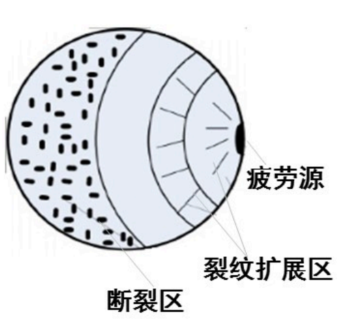
\includegraphics[width=0.7\textwidth]{Figure/疲劳破坏过程.png}
\caption{疲劳破坏过程}
\label{fig:疲劳破坏过程}
\end{figure}

\subsubsection{疲劳破坏特征}

\begin{definition}[疲劳破坏特征]
\label{def:疲劳破坏特征}
\begin{enumerate}
	\item \textbf{断裂过程}：（1）产生微观初始裂纹；（2）裂纹尖端在切应力作用下反复扩展，直至产生宏观疲劳裂纹；（3）达到临界尺寸后突然断裂。
	\item \textbf{断裂面}：（1）光滑区（疲劳发展区）；（2）粗糙区（脆性断裂区）。
	\item 无明显塑性变形的\textcolor{red}{脆性突然断裂}。
	\item 破坏时的应力（疲劳极限）\textbf{远小于}屈服极限。
\end{enumerate}
\end{definition}

\subsubsection{疲劳破坏的机理与影响因素}

\begin{definition}[疲劳破坏的机理与影响因素]
\label{def:疲劳破坏机理}
\textbf{疲劳破坏的机理}：损伤的累积。

\textbf{影响因素}：应力循环次数、变应力的循环特性、应力幅，还与材料抗疲劳性能有关。当 $\sigma_m$、$\gamma$ 一定时，$\sigma_a$ 越小，材料寿命越长（极限循环次数 $N$ 越大），越不容易产生疲劳破坏。
\end{definition}

\begin{note}
课件原文此处写作"$\sigma_a$ 越小，$N$ 越少"，与疲劳曲线规律（应力幅越小、寿命越长）相反，笔记按正确结论"$N$ 越大"记录。
\end{note}

\subsection{材料的疲劳曲线和疲劳极限}

\begin{definition}[疲劳极限]
\label{def:疲劳极限}
\textbf{疲劳极限} $\sigma_{\gamma N}$（$\tau_{\gamma N}$）：循环变应力下，应力循环 $N$ 次后材料不发生疲劳破坏时的最大应力。
\end{definition}

\begin{definition}[疲劳寿命]
\label{def:疲劳寿命}
\textbf{疲劳寿命} $N$：材料疲劳失效前所经历的应力循环次数。
\end{definition}

\begin{definition}[疲劳曲线]
\label{def:疲劳曲线}
\textbf{疲劳曲线}：应力循环特性 $\gamma$ 一定时，材料的疲劳极限与应力循环次数之间的关系曲线。其中 $N_0$ 为\textbf{循环基数}（$(10\sim25)\times10^7$），$\sigma_\gamma$ 为\textbf{持久极限}。
\end{definition}

\begin{figure}[H]
\centering
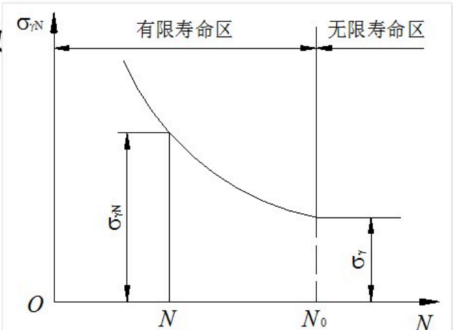
\includegraphics[width=0.7\textwidth]{Figure/疲劳曲线.png}
\caption{材料的疲劳曲线}
\label{fig:疲劳曲线}
\end{figure}

\textbf{（1）有限寿命区} $N<N_0$：
\begin{itemize}
	\item 低周循环疲劳 $N<10^3(10^4)$：疲劳极限接近于屈服极限，按静强度计算。如压力容器、火箭发动机的某些零件等。
	\item 高周循环疲劳 $N\ge10^3(10^4)$：如弹簧、传动轴等；\textbf{随循环次数$\uparrow$，疲劳极限$\downarrow$}。
\end{itemize}

\textbf{（2）无限寿命区} $N\ge N_0$：$\sigma_{\gamma N}=\sigma_\gamma$（持久极限）。
\begin{itemize}
	\item 对称循环：$\sigma_{-1}$、$\tau_{-1}$；脉动循环：$\sigma_0$、$\tau_0$。
	\item 注意：\textbf{有色金属和高强度合金钢无无限寿命区}。
\end{itemize}

\begin{theorem}[疲劳曲线方程]
\label{thm:疲劳曲线方程}
\begin{equation}
	\sigma_{\gamma N}^m \cdot N = \sigma_\gamma^m \cdot N_0 = C
	\label{eq:强度:疲劳曲线方程}
\end{equation}
\begin{equation}
	\therefore\quad \sigma_{\gamma N}=\sqrt[m]{\frac{N_0}{N}}\,\sigma_\gamma = K_N\cdot\sigma_\gamma
	\label{eq:强度:疲劳极限有限寿命}
\end{equation}
\begin{equation}
	K_N=\sqrt[m]{\frac{N_0}{N}}\quad\text{——寿命系数}
	\label{eq:强度:寿命系数}
\end{equation}
采用寿命系数，通过疲劳曲线方程，可计算任意循环次数 $N$ 下的疲劳极限应力 $\sigma_{\gamma N}$。
\end{theorem}

\begin{note}
\begin{enumerate}
	\item $N_0$：硬度 $\le350\,\text{HBS}$ 钢，$N_0=10^7$；$\ge350\,\text{HBS}$ 钢，$N_0=(10\sim25)\times10^7$；有色金属（无水平部分）规定当 $N>25\times10^7$ 时取 $N=N_0=25\times10^7$ 近似为无限寿命区。
	\item $m$——指数与应力和材料种类有关。钢 $m=9$（拉、弯应力，剪应力）、$m=6$（接触应力）；青铜 $m=9$（弯曲应力）、$m=8$（接触应力）。
	\item 应力循环特性 $\gamma$ 越大，材料的疲劳极限与持久极限越高，对零件强度越有利；\textbf{对称循环（$\gamma=-1$）最不利}。
\end{enumerate}
\end{note}

\subsection{材料的疲劳极限应力图（$\sigma_m-\sigma_a$ 图）}

同一种材料（标准试件）在不同的应力循环特性下进行疲劳试验，可得到持久极限 $\sigma_\gamma$（即 $\sigma_{\max}$）；由应力循环特性可求出 $\sigma_{\min}=\gamma\sigma_{\max}$ 和 $\sigma_m$、$\sigma_a$；以 $\sigma_m$ 为横坐标、$\sigma_a$ 为纵坐标，即得材料在不同应力循环特性下的极限 $\sigma_m$ 和 $\sigma_a$ 的关系图。

\begin{definition}[材料的疲劳极限应力图]
\label{def:材料的疲劳极限应力图}
\textbf{塑性材料的疲劳极限应力图呈抛物线分布（$A'B$ 曲线）}。四个特征点为：
\begin{itemize}
	\item $A'(0,\ \sigma_{-1})$ —— 对称疲劳极限点；
	\item $D'(\sigma_0/2,\ \sigma_0/2)$ —— 脉动疲劳极限点；
	\item $B(\sigma_B,\ 0)$ —— 强度极限点；
	\item $C(\sigma_s,\ 0)$ —— 屈服极限点。
\end{itemize}
曲线上的点对应着不同应力循环特性下材料的疲劳极限 $\sigma_\gamma$。
\end{definition}

\begin{figure}[H]
\centering
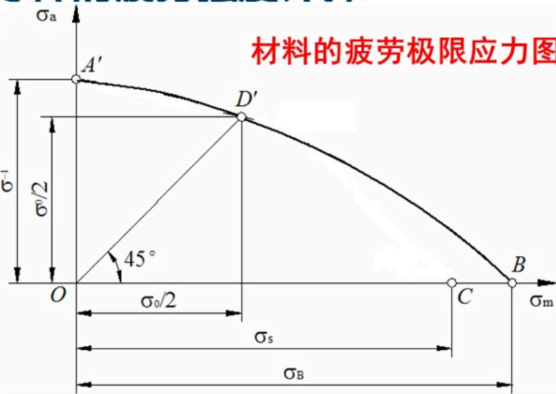
\includegraphics[width=0.7\textwidth]{Figure/材料的疲劳极限应力图.png}
\caption{材料的疲劳极限应力图}
\label{fig:材料的疲劳极限应力图}
\end{figure}

\begin{definition}[简化疲劳极限应力图]
\label{def:简化疲劳极限应力图}
考虑塑性材料的最大应力不超过屈服极限，由 $C$ 点作 $135°$ 斜线与 $A'D'$ 的延长线交于 $G'$，得到折线 $\boldsymbol{A'D'G'C}$。
\begin{itemize}
	\item 折线上各点的横坐标——极限平均应力 $\sigma_m'$；纵坐标——极限应力幅 $\sigma_a'$。
	\item $G'C$ 上各点：$\sigma_{\max}'=\sigma_m'+\sigma_a'=\sigma_s$，若 $\sigma_{\max}<\sigma_s$ 不会屈服破坏。
	\item 折线\textbf{以内}——疲劳和塑性安全区；\textbf{以外}——疲劳和塑性失效区。
	\item 零件工作应力点 $(\sigma_m,\ \sigma_a)$ 应位于 $A'D'G'C$ 以内。
\end{itemize}
\end{definition}

\begin{figure}[H]
\centering
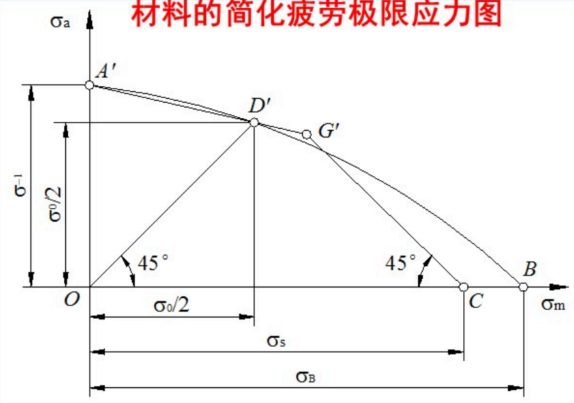
\includegraphics[width=0.7\textwidth]{Figure/材料的简化疲劳极限应力图.png}
\caption{材料的简化疲劳极限应力图}
\label{fig:材料的简化疲劳极限应力图}
\end{figure}

\subsection{影响机械零件疲劳强度的主要因素和零件极限应力图}

实际机械零件与标准试件之间有差异，使零件的疲劳极限不同于材料的疲劳极限，其中尤以\textcolor{red}{应力集中、零件尺寸和表面状态}对机械零件的疲劳强度影响最大。

\subsubsection{应力集中的影响——有效应力集中系数 $k_\sigma(k_\tau)$}

零件受载时，在几何形状突变处（圆角、凹槽、孔等）产生应力集中。材料强度越高、硬度越高，对应力集中越敏感。

\begin{definition}[有效应力集中系数 $k_\sigma(k_\tau)$]
\label{def:有效应力集中系数}
\textbf{有效应力集中系数}为
\begin{equation}
	k_\sigma=1+q_\sigma(\alpha_\sigma-1)
	\label{eq:强度:有效应力集中系数}
\end{equation}
其中，$q_\sigma$ 为材料的敏感系数。
\end{definition}

\begin{definition}[理论应力集中系数]
\label{def:理论应力集中系数}
\textbf{理论应力集中系数}为
\begin{equation}
	\alpha_\sigma=\frac{\sigma_{\max}}{\sigma}
	\label{eq:强度:理论应力集中系数}
\end{equation}
其中，$\sigma_{\max}$ 为实际最大应力，$\sigma$ 为名义应力。
\end{definition}

\subsubsection{零件尺寸的影响——尺寸系数 $\varepsilon_\sigma(\varepsilon_\tau)$}

\begin{definition}[尺寸系数 $\varepsilon_\sigma(\varepsilon_\tau)$]
\label{def:尺寸系数}
\textbf{尺寸系数}反映零件尺寸对疲劳强度的影响：零件尺寸愈大时，材料的晶粒较粗、出现缺陷的概率大，而机械加工后表面冷作硬化层相对较薄，所以对零件疲劳强度的不良影响愈显著。
\end{definition}

\subsubsection{表面状态的影响}

\begin{definition}[表面状态的影响因素]
\label{def:表面状态}
表面状态的影响因素有：表面加工质量、表面强化处理工艺和表面腐蚀状况等。
\begin{enumerate}
	\item \textbf{表面质量系数 $\beta_1$}：零件加工的表面质量（主要指表面粗糙度）对疲劳强度的影响。钢的 $\sigma_B$ 越高、表面愈粗糙，$\beta_1$ 愈低。
	\item \textbf{表面强化系数 $\beta_2$}：考虑对零件进行不同的强化处理（淬火、渗氮、渗碳等热处理工艺；抛光、喷丸、滚压等冷作工艺）对疲劳强度的影响。
	\item \textbf{表面腐蚀系数 $\beta_3$}：受到腐蚀的零件表面会产生腐蚀垢，形成应力集中源，故腐蚀也会降低零件的疲劳强度。
\end{enumerate}
\end{definition}

\textbf{表面系数 $\beta$ 的取值}：

\begin{table}[H]
\centering
\caption{表面系数 $\beta$ 的取值}
\label{tab:强度:表面系数}
\begin{tabular}{cl}
	\toprule
	工作状态 & $\beta$ 取值 \\
	\midrule
	零件只经过切削 & $\beta=\beta_1$ \\
	零件切削后又强化处理 & $\beta=\beta_2$ \\
	零件在腐蚀介质中工作 & $\beta=\beta_3$ \\
	\bottomrule
\end{tabular}
\end{table}

\subsubsection{综合影响系数 $K_\sigma(K_\tau)$ 和零件的极限应力图}

应力集中、零件尺寸和表面状态 $k_\sigma,\varepsilon_\sigma,\beta$ 只对应力幅 $\sigma_a$ 有影响，而对平均应力 $\sigma_m$ 无影响（由试验得）。

\begin{theorem}[综合影响系数]
\label{thm:综合影响系数}
\begin{equation}
	K_\sigma=\frac{k_\sigma}{\varepsilon_\sigma\beta_\sigma},\qquad K_\tau=\frac{k_\tau}{\varepsilon_\tau\beta_\tau}
	\label{eq:强度:综合影响系数}
\end{equation}
综合影响系数表示了\textbf{材料极限应力幅与零件极限应力幅的比值}：
\begin{equation}
	K_\sigma=\frac{\sigma_a'\,(\text{标准试件的极限应力幅})}{\sigma_{ae}'\,(\text{零件的极限应力幅})}
	\label{eq:强度:综合影响系数比值1}
\end{equation}
对称循环：
\begin{equation}
	K_\sigma=\frac{\sigma_{-1}\,(\text{标准试件对称循环的疲劳极限})}{\sigma_{-1e}\,(\text{零件试件对称循环的疲劳极限})}
	\label{eq:强度:综合影响系数比值2}
\end{equation}
\end{theorem}

\begin{definition}[零件的极限应力图]
\label{def:零件的极限应力图}
由于 $K_\sigma$ 只对 $\sigma_a$ 有影响、对 $\sigma_m$ 无影响，所以在材料极限应力图 $A'D'G'C$ 的纵坐标上计入 $K_\sigma$ 的影响：
\begin{itemize}
	\item $A\left(0,\ \dfrac{\sigma_{-1}}{K_\sigma}\right)$ —— 零件对称循环疲劳点；
	\item $D\left(\dfrac{\sigma_0}{2},\ \dfrac{\sigma_0}{2K_\sigma}\right)$ —— 零件脉动循环疲劳点。
\end{itemize}
得到零件的许用疲劳极限曲线（$A\!-\!D\!-\!G$ 折线）与屈服极限曲线（$G\!-\!C$）。
\end{definition}

\begin{figure}[H]
\centering
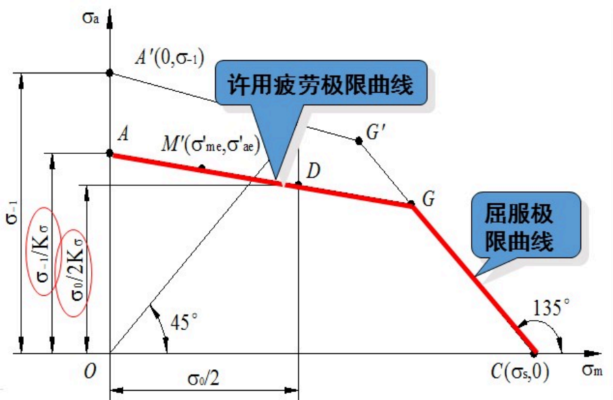
\includegraphics[width=0.7\textwidth]{Figure/零件的极限应力图.png}
\caption{零件的极限应力图}
\label{fig:零件的极限应力图}
\end{figure}

\begin{theorem}[零件极限应力图的直线方程]
\label{thm:极限应力图直线方程}
直线 $CG$ 方程：
\begin{equation}
	\sigma_{ae}'+\sigma_{me}'=\sigma_s
	\label{eq:强度:零件CG直线}
\end{equation}
直线 $AG$ 方程：
\begin{equation}
	\sigma_{-1e}=\frac{\sigma_{-1}}{K_\sigma}=\sigma_{ae}'+\left(\frac{1}{K_\sigma}\cdot\frac{2\sigma_{-1}-\sigma_0}{\sigma_0}\right)\sigma_{me}'
	\label{eq:强度:零件AG直线}
\end{equation}
即
\begin{equation}
	\sigma_{-1}=K_\sigma\sigma_{ae}'+\frac{2\sigma_{-1}-\sigma_0}{\sigma_0}\,\sigma_{me}'
	\label{eq:强度:材料AG直线}
\end{equation}
其中，$\psi_\sigma=\dfrac{2\sigma_{-1}-\sigma_0}{\sigma_0}$ 为标准试件的材料特性；$\psi_{\sigma e}=\dfrac{\psi_\sigma}{K_\sigma}$ 为零件的材料特性。
\end{theorem}

\subsection{单向稳定变应力时的疲劳强度计算}

\textbf{计算步骤（流程）}：
\begin{enumerate}
	\item 先画出材料的极限应力图；
	\item 查出并计算零件的综合影响系数；
	\item 画出零件的极限应力图；
	\item 找到工作应力点；
	\item 找到与之对应的极限应力点；
	\item 求出最大极限应力；
	\item 最后求安全系数。
\end{enumerate}

\subsubsection{$\gamma = \dfrac{\sigma_{\min}}{\sigma_{\max}} = C$}

大多数转轴中的主应力状态（承受扭矩和弯矩的轴），满足
\begin{equation}
	\frac{\sigma_a}{\sigma_m}=\frac{1-\gamma}{1+\gamma}=\text{常数}
	\label{eq:强度:gamma等于C}
\end{equation}
过原点与工作应力点 $M$（或 $N$）作连线交 $ADG$（或 $GC$）于 $M_1'$（$N_1'$）点，直线上任一点的应力循环特性均相同，$M_1'$、$N_1'$ 即为\textbf{极限应力点}。

\begin{theorem}[$\gamma=C$ 时的疲劳强度计算]
\label{thm:gammaC}
\textbf{a) 工作应力点位于 $OAG$ 内}：极限应力为疲劳极限，按疲劳强度计算。
\begin{equation}
	\sigma_{\mathrm{lime}}=\sigma_{\max}'=\sigma_{ae}'+\sigma_{me}'=\frac{\sigma_{-1}(\sigma_m+\sigma_a)}{K_\sigma\sigma_a+\psi_\sigma\sigma_m}=\frac{\sigma_{-1}\sigma_{\max}}{K_\sigma\sigma_a+\psi_\sigma\sigma_m}
	\label{eq:强度:gammaC极限应力}
\end{equation}
强度条件为：
\begin{equation}
	S_{ca}=\frac{\sigma_{\mathrm{lime}}}{\sigma_{\max}}=\frac{\sigma_{-1}}{K_\sigma\sigma_a+\psi_\sigma\sigma_m}\ge[S]
	\label{eq:强度:gammaC疲劳}
\end{equation}

\textbf{b) 工作应力点位于 $OGC$ 内}：极限应力为屈服极限，按静强度计算。
\begin{equation}
	S_{ca}=\frac{\sigma_s}{\sigma_{\max}}=\frac{\sigma_s}{\sigma_m+\sigma_a}\ge[S]
	\label{eq:强度:gammaC屈服}
\end{equation}
\end{theorem}

\subsubsection{$\sigma_m = C$}

振动中的受载弹簧的应力状态。过工作应力点 $M$（$N$）作与纵轴平行的直线交 $AGC$ 于 $M_2'$（$N_2'$）点，即为极限应力点。

\begin{theorem}[$\sigma_m=C$ 时的疲劳强度计算]
\label{thm:sigmaM}
\textbf{a) 工作应力点位于 $OAGH$ 区域}：极限应力为疲劳极限。
\begin{equation}
	\sigma_{\mathrm{lime}}=\sigma_{\max}'=\sigma_{me}'+\sigma_{ae}'=\sigma_m+\frac{\sigma_{-1}-\psi_\sigma\sigma_m}{K_\sigma}
	\label{eq:强度:sigmaM极限应力}
\end{equation}
强度条件为：
\begin{equation}
	S_{ca}=\frac{\sigma_{-1}+(K_\sigma-\psi_\sigma)\sigma_m}{K_\sigma(\sigma_m+\sigma_a)}\ge[S]
	\label{eq:强度:sigmaM疲劳}
\end{equation}

\textbf{b) 工作应力点位于 $GHC$ 区域}：极限应力为屈服极限。
\begin{equation}
	S_{ca}=\frac{\sigma_s}{\sigma_{\max}}=\frac{\sigma_s}{\sigma_m+\sigma_a}\ge[S]
	\label{eq:强度:sigmaM屈服}
\end{equation}
\end{theorem}

\subsubsection{$\sigma_{\min} = C$}

受轴向变载荷的紧螺栓联接中的螺栓应力状态，满足
\begin{equation}
	\sigma_{\min}=\sigma_m-\sigma_a=C
	\label{eq:强度:sigmaMin等于C}
\end{equation}
过工作应力点 $M$（$N$）作与横坐标成 $45°$ 的直线，直线与极限应力线图的交点 $M_3'$（$N_3'$）即为所求极限应力点。

\begin{theorem}[$\sigma_{\min}=C$ 时的疲劳强度计算]
\label{thm:sigmaMin}
\textbf{a) 工作应力点位于 $OJGI$ 区域}：极限应力为疲劳极限。
\begin{equation}
	\sigma_{\mathrm{lime}}=\sigma_{\max}'=\sigma_{ae}'+\sigma_{me}'=\frac{2\sigma_{-1}+(K_\sigma-\psi_\sigma)\sigma_{\min}}{K_\sigma+\psi_\sigma}
	\label{eq:强度:sigmaMin极限应力}
\end{equation}
强度条件为：
\begin{equation}
	S_{ca}=\frac{\sigma_{\mathrm{lime}}}{\sigma_{\max}}=\frac{2\sigma_{-1}+(K_\sigma-\psi_\sigma)\sigma_{\min}}{(K_\sigma+\psi_\sigma)(\sigma_m+\sigma_a)}=\frac{2\sigma_{-1}+(K_\sigma-\psi_\sigma)\sigma_{\min}}{(K_\sigma+\psi_\sigma)(2\sigma_a+\sigma_{\min})}\ge[S]
	\label{eq:强度:sigmaMin疲劳}
\end{equation}

\textbf{b) 工作应力点位于 $IGC$ 区域}：极限应力为屈服极限，按静强度计算。
\begin{equation}
	S_{ca}=\frac{\sigma_s}{\sigma_{\max}}=\frac{\sigma_s}{\sigma_m+\sigma_a}=\frac{\sigma_s}{\sigma_{\min}+2\sigma_a}\ge[S]
	\label{eq:强度:sigmaMin屈服}
\end{equation}

\textbf{c) 工作应力位于 $0AJ$ 区域内}：$\sigma_{\min}$ 为负值，工程中罕见，故不作考虑。
\end{theorem}

\begin{note}
\begin{enumerate}
	\item 若零件所受应力变化规律不能肯定，一般采用 $\gamma=C$ 的情况计算；
	\item 上述计算均按\textbf{无限寿命}设计。若按\textbf{有限寿命}要求设计（$10^3(10^4)<N<N_0$），公式中的极限应力应为有限寿命的疲劳极限 $\sigma_{\gamma N}=\sqrt[m]{\dfrac{N_0}{N}}\,\sigma_\gamma$，即以 $\sigma_{-1N}$ 代 $\sigma_{-1}$、以 $\sigma_{0N}$ 代 $\sigma_0$；
	\item 当未知工作应力点所在区域时，应同时考虑可能出现的两种情况；
	\item 对切应力上述公式同样适用，只需将 $\sigma$ 改为 $\tau$ 即可。
\end{enumerate}
\end{note}

\subsubsection{例题 1（课件原题）}

\begin{longexample}[单向稳定变应力疲劳强度校核]
\label{ex:单向疲劳校核}
某轴受弯曲稳定变应力作用，$\sigma_{\max}=260\ \mathrm{MPa}$，$\sigma_{\min}=-60\ \mathrm{MPa}$。已知 $\sigma_{-1}=450\ \mathrm{MPa}$，$\sigma_0=700\ \mathrm{MPa}$，$\sigma_s=800\ \mathrm{MPa}$，弯曲疲劳极限的综合影响系数 $K_\sigma=1.9$。

（1）绘制材料的简化极限应力图，在图中标出工作应力点，并判别其可能破坏的形式；
（2）按许用安全系数 $[S]=1.4$，校核此轴的无限寿命疲劳强度；
（3）若轴的转速 $n=20\ \mathrm{r/min}$，每天工作 8 小时，共工作 360 天，循环基数 $N_0=5\times10^6$，寿命指数 $m=9$，按有限寿命校核其疲劳强度，$[S]=1.4$。

\begin{solution}
\textbf{（1）}求工作应力点坐标：
\begin{equation}
	\sigma_a=\frac{\sigma_{\max}-\sigma_{\min}}{2}=\frac{260-(-60)}{2}=160\ \mathrm{MPa}
	\label{eq:强度:例1应力幅}
\end{equation}
\begin{equation}
	\sigma_m=\frac{\sigma_{\max}+\sigma_{\min}}{2}=\frac{260+(-60)}{2}=100\ \mathrm{MPa}
	\label{eq:强度:例1平均应力}
\end{equation}
\begin{itemize}
	\item 工作应力点 $N(100,\ 160)$；
	\item 极限应力图特征点：$A(0,\ 450)$（$\sigma_{-1}$）、$D'(350,\ 350)$（$\sigma_0/2,\sigma_0/2$）、$C(800,\ 0)$（$\sigma_s$）；
	\item $\gamma=\dfrac{\sigma_{\min}}{\sigma_{\max}}=\dfrac{-60}{260}\approx-0.23$，属 $\gamma=C$ 情形；
	\item 判别：$\psi_\sigma=\dfrac{2\sigma_{-1}-\sigma_0}{\sigma_0}=\dfrac{200}{700}\approx0.286$，直线 $AG$ 上 $\sigma_m=100$ 处 $\sigma_a'=\dfrac{\sigma_{-1}}{K_\sigma}-\dfrac{\psi_\sigma}{K_\sigma}\sigma_m=\dfrac{450}{1.9}-\dfrac{0.286}{1.9}\times100\approx221.8>160$，工作应力点位于\textbf{$OAG$ 区域内}，可能发生\textbf{疲劳破坏}。
\end{itemize}

\textbf{（2）}按 $\gamma=C$ 计算，无限寿命：
\begin{equation}
	\psi_\sigma=\frac{2\sigma_{-1}-\sigma_0}{\sigma_0}=\frac{2\times450-700}{700}\approx0.286
	\label{eq:强度:例1psi}
\end{equation}
\begin{equation}
	S_{ca}=\frac{\sigma_{-1}}{K_\sigma\sigma_a+\psi_\sigma\sigma_m}=\frac{450}{1.9\times160+0.286\times100}=\frac{450}{332.6}\approx1.35<1.4
	\label{eq:强度:例1无限寿命}
\end{equation}
故按无限寿命校核\textbf{不安全}。

\textbf{（3）}应力循环次数：
\begin{equation}
	N=60nt=60\times20\times8\times360=3.456\times10^6
	\label{eq:强度:例1循环次数}
\end{equation}
寿命系数：
\begin{equation}
	K_N=\sqrt[9]{\frac{N_0}{N}}=\sqrt[9]{\frac{5\times10^6}{3.456\times10^6}}\approx1.04
	\label{eq:强度:例1寿命系数}
\end{equation}
\begin{equation}
	\sigma_{-1N}=K_N\sigma_{-1}
	\label{eq:强度:例1疲劳极限}
\end{equation}
\begin{equation}
	S_{ca}=\frac{\sigma_{-1N}}{K_\sigma\sigma_a+\psi_\sigma\sigma_m}=\frac{K_N\sigma_{-1}}{K_\sigma\sigma_a+\psi_\sigma\sigma_m}\approx1.04\times1.35\approx1.4\ge1.4
	\label{eq:强度:例1有限寿命}
\end{equation}
故按有限寿命校核\textbf{安全}。
\end{solution}
\end{longexample}

\subsection{双向稳定变应力时的疲劳强度计算}

弯扭联合作用、拉扭联合作用。当零件上同时作用有\textbf{同相位}的对称循环变应力 $\sigma_a$ 和 $\tau_a$ 时，钢材满足以下极限应力关系式：

\begin{theorem}[双向稳定变应力的强度条件]
\label{thm:双向}
\begin{equation}
	\left(\frac{\tau_a'}{\tau_{-1e}}\right)^2+\left(\frac{\sigma_a'}{\sigma_{-1e}}\right)^2=1
	\label{eq:强度:椭圆方程}
\end{equation}
其中，$\tau_{-1e}$、$\sigma_{-1e}$ 为零件受对称循环的疲劳极限；$\tau_a'$、$\sigma_a'$ 为同时承受双向应力时的应力幅的极限值。

\textbf{推导}：由 $S_{ca}=\dfrac{OM'}{OM}=\dfrac{OC'}{OC}=\dfrac{OD'}{OD}$，有
\begin{equation}
	\tau_a'=S_{ca}\tau_a,\qquad \sigma_a'=S_{ca}\sigma_a
	\label{eq:强度:双向应力幅}
\end{equation}
令 $S_\tau=\dfrac{\tau_{-1e}}{\tau_a}$，$S_\sigma=\dfrac{\sigma_{-1e}}{\sigma_a}$，代入椭圆方程得：
\begin{equation}
	\left(\frac{S_{ca}}{S_\tau}\right)^2+\left(\frac{S_{ca}}{S_\sigma}\right)^2=1
	\label{eq:强度:双向椭圆方程}
\end{equation}
最终强度条件：
\begin{equation}
	S_{ca}=\frac{S_\sigma S_\tau}{\sqrt{S_\sigma^2+S_\tau^2}}\ge[S]
	\label{eq:强度:双向安全系数}
\end{equation}
\end{theorem}

\section{机械零件的接触强度}
\label{sec:接触强度}

\begin{definition}[接触应力与接触强度]
\label{def:接触应力与接触强度}
高副零件工作时，理论上是点接触或线接触→实际上由于接触部分的局部弹性变形而形成面接触→由于接触面积很小，使表层产生的局部应力却很大，该应力称为\textbf{接触应力}。在表面接触应力作用下的零件强度称为\textbf{接触强度}。计算依据是弹性力学的\textbf{赫兹公式}。
\end{definition}

\subsection{接触应力}

\subsubsection{两圆柱体接触}

\begin{theorem}[两圆柱体接触应力（赫兹公式）]
\label{thm:两圆柱接触}
\begin{equation}
	\sigma_H=\sqrt{\frac{F\left(\dfrac{1}{\rho_\Sigma}\right)}{\pi b\left[\left(\dfrac{1-\mu_1^2}{E_1}\right)+\left(\dfrac{1-\mu_2^2}{E_2}\right)\right]}}
	\label{eq:强度:两圆柱接触应力}
\end{equation}
当 $\mu_1=\mu_2=0.3,\ E_1=E_2=E$ 时：
\begin{equation}
	\sigma_{H\max}=0.418\sqrt{\frac{FE}{b\rho_\Sigma}}
	\label{eq:强度:两圆柱接触应力简化}
\end{equation}
\end{theorem}

\begin{figure}[H]
\centering
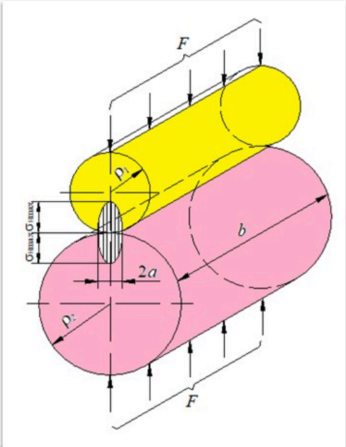
\includegraphics[width=0.7\textwidth]{Figure/两圆柱接触应力.png}
\caption{两圆柱体接触应力}
\label{fig:两圆柱接触应力}
\end{figure}

\subsubsection{两球接触}

\begin{theorem}[两球接触应力（赫兹公式）]
\label{thm:两球接触}
\begin{equation}
	\sigma_{H\max}=\frac{1}{\pi}\sqrt[3]{6F\left[\frac{\dfrac{1}{\rho_\Sigma}}{\dfrac{1-\mu_1^2}{E_1}+\dfrac{1-\mu_2^2}{E_2}}\right]^2}
	\label{eq:强度:两球接触应力}
\end{equation}
当 $\mu_1=\mu_2=0.3,\ E_1=E_2=E$ 时：
\begin{equation}
	\sigma_{H\max}=0.388\sqrt[3]{\frac{FE^2}{\rho_\Sigma^2}}
	\label{eq:强度:两球接触应力简化}
\end{equation}
\end{theorem}

\begin{definition}[综合曲率半径]
\label{def:综合曲率半径}
$\rho_\Sigma$ 为\textbf{综合曲率半径}：
\begin{equation}
	\frac{1}{\rho_\Sigma}=\frac{1}{\rho_1}\pm\frac{1}{\rho_2}\quad\begin{cases}+\rightarrow\text{外接触}\\-\rightarrow\text{内接触}\end{cases}
	\label{eq:强度:综合曲率半径}
\end{equation}
\end{definition}

\begin{figure}[H]
\centering
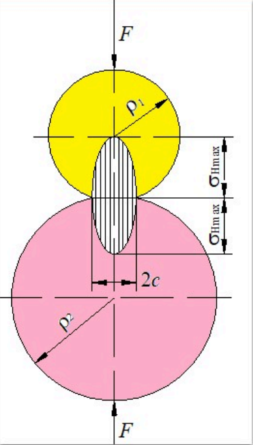
\includegraphics[width=0.7\textwidth]{Figure/两球体接触应力.png}
\caption{两球体接触应力}
\label{fig:两球体接触应力}
\end{figure}

\begin{note}
\begin{enumerate}
	\item 圆柱体 $\sigma_{H\max}\propto F^{1/2}$，球 $\sigma_{H\max}\propto F^{1/3}$，$\therefore \sigma_{H\max}$ 与 $F$ \textbf{不呈线性关系}。
	\item 圆柱体 $\sigma_{H\max}\propto\dfrac{1}{\rho_\Sigma^{1/2}}$，球 $\sigma_{H\max}\propto\dfrac{1}{\rho_\Sigma^{2/3}}$，$\therefore \rho_\Sigma$ 越大，$\sigma_{H\max}$ 越小。
	\item 同样的 $\rho_1$、$\rho_2$ 下，\textbf{内接触时 $\rho_\Sigma$ 较大、$\sigma_{H\max}$ 较小}，约为外接触时的 48%。∴ 重载情况下采用内接触，有利于提高承载能力或降低接触副的尺寸。
\end{enumerate}
\end{note}

\subsection{失效形式}

\begin{definition}[接触强度失效形式]
\label{def:接触失效形式}
\begin{itemize}
	\item \textbf{静应力}：表面压碎（脆性材料）；表面塑性变形（塑性材料）。
	\item \textbf{变应力}：\textbf{疲劳点蚀}——齿轮、滚动轴承的常见失效形式。
\end{itemize}
\end{definition}

\subsection{提高接触疲劳强度的措施}

接触强度条件为 $\sigma_{H\max}\le[\sigma]_H$：
\begin{enumerate}
	\item 控制最大接触应力；
	\item 提高接触表面硬度，改善表面加工质量；
	\item 增大综合曲率半径 $\rho_\Sigma$；
	\item 改外接触为内接触，点接触→线接触；
	\item 采用高粘度润滑油。
\end{enumerate}

\section*{本章重点}
\addcontentsline{toc}{section}{本章重点}

\begin{enumerate}
	\item \textbf{应力的分类}：对称循环、脉动循环；
	\item \textbf{材料极限应力图}和\textbf{零件极限应力图}；
	\item 影响机械零件疲劳强度的主要因素（应力集中、零件尺寸、表面状态）；
	\item \textbf{单向稳定变应力时的疲劳强度计算}：$\gamma=C$，$\sigma_m=C$，$\sigma_{\min}=C$ 三种情况；
	\item 影响机械零件接触应力的主要因素。
\end{enumerate}
